\chapter{Advanced Linear Algebra: The Secret Superpowers of Matrices}

% ============================================
% TikZ Style Definitions - Simple and Readable (matching Chapter 1)
% ============================================
\tikzset{
    % Axis styles - dark enough to read
    axis/.style={->, thick, black!60},
    axis label/.style={font=\footnotesize, black!70},
    % Grid styles
    grid/.style={very thin, black!15},
    % Vector styles - bold colors
    vec blue/.style={->, very thick, blue!80!black},
    vec red/.style={->, very thick, red!70!black},
    vec green/.style={->, very thick, green!50!black},
    vec purple/.style={->, very thick, purple!70!black},
    vec orange/.style={->, very thick, orange!70!black},
    % Eigenvalue specific styles (for this chapter)
    eigen vec/.style={->, very thick},
    % Label styles - simple and readable
    vec label/.style={font=\footnotesize},
    title label/.style={font=\footnotesize\bfseries},
    % Info box for labels
    info box/.style={font=\footnotesize, inner sep=2pt},
    % Dashed helper lines
    helper/.style={dashed, black!40, thin},
}

\begin{center}
\textit{``Eigen'' is German for ``own'' or ``characteristic.'' So eigenvectors are a matrix's ``own'' special vectors. Germans really know how to name things.}

\vspace{0.3cm}

\textit{``The eigenvectors are the skeleton of the matrix---everything else is just flesh.''} --- A professor who really loved linear algebra
\end{center}

\vspace{0.5cm}

In Chapter 1, you learned that matrices are transformations---they stretch, rotate, shear, and project vectors. But we treated matrices as mysterious black boxes. Put a vector in, get a vector out, hope for the best.

Now it's time to crack open the black box.

This chapter is about discovering the \textbf{hidden structure} inside every matrix. We'll find secret directions, hidden scaling factors, and learn to decompose any matrix into its fundamental building blocks. By the end, you'll be able to look at a matrix and understand \textit{what it really does}---not just compute with it, but truly see it.

\begin{connection}
\textbf{Why This Chapter Will Change How You See AI}

The concepts in this chapter aren't just abstract math---they're the foundation of:
\begin{itemize}
    \item \textbf{Principal Component Analysis (PCA):} How we reduce 1000-dimensional data to something visualizable
    \item \textbf{Google's PageRank:} The algorithm that made Google Google (it's an eigenvector!)
    \item \textbf{LoRA fine-tuning:} How we adapt giant LLMs with minimal resources (SVD in disguise)
    \item \textbf{Understanding training dynamics:} Why some neural networks train smoothly and others explode
    \item \textbf{Image/video compression:} Why your Netflix stream doesn't buffer (much)
    \item \textbf{Recommendation systems:} How Spotify knows you'll love that obscure indie band
\end{itemize}

If Chapter 1 taught you the alphabet, this chapter teaches you to read poetry.
\end{connection}

\section{The Mystery of the Special Directions}

\subsection{A Puzzle to Start}

Imagine you have a magical Instagram filter. When you apply it to a picture, most things get warped---faces stretch, buildings lean, colors shift in weird ways. Your carefully composed selfie becomes abstract art (and not in a good way).

But here's the weird part: \textit{some} parts of the image just get brighter or darker without changing shape at all. They refuse to warp. They're stubborn like that.

Those unchanged directions? They're special. They're the filter's ``natural axes.'' And in the world of matrices, we call them \textbf{eigenvectors}. (Pronounced ``EYE-gen-vectors,'' not ``egg-en-vectors.'' You're welcome.)

This chapter is about finding those special directions and understanding why they matter so much for AI. Spoiler alert: They're the key to understanding how neural networks learn, how data compresses, and how Netflix knows you'll love that obscure documentary about competitive dog grooming.

\begin{intuition}
\textbf{The Treasure Map Analogy}

Imagine you're given a treasure map, but it's in a foreign language and uses a weird coordinate system. You could try to follow it directly (hard), or you could:
\begin{enumerate}
    \item Translate it to English (change of basis)
    \item Convert to North/South/East/West (natural coordinates)
    \item Walk straight to the treasure (simple path)
\end{enumerate}

That's what eigenvectors do for matrices! They find the ``natural coordinate system'' where everything becomes simple. Instead of a complicated transformation with spinning and stretching and shearing, you get pure scaling along nice perpendicular axes.

\textbf{This is the central theme of this chapter:} Finding the right perspective makes hard problems easy.
\end{intuition}

\section{Eigenvectors: The Vectors That Refuse to Turn}

\subsection{The Big Idea (No Math Yet, Just Vibes)}

Most of the time, when you multiply a matrix by a vector, the vector spins around, changes direction, gets warped into something unrecognizable. It's chaos. It's a vector having a bad day.

But sometimes---\textit{sometimes}---you find a vector that's so perfectly aligned with what the matrix ``wants to do'' that it just gets stretched or shrunk, without rotating at all. It's like the vector found the matrix's secret shortcut.

\textbf{Real-world analogies (because math needs friends):}

\textbf{The Shopping Cart:} You're pushing a shopping cart with one wonky wheel. Most directions require constant course correction---you push forward, but the cart veers left. But there's ONE magical direction where the cart rolls perfectly straight. That's an eigendirection!

\textbf{The Rubber Band Grid:} Stretch a grid made of rubber bands. Most points move in complicated diagonal ways. But the vertical and horizontal directions? They just stretch along themselves, nice and simple. Those are eigendirections!

\textbf{The Lazy River:} Imagine a lazy river at a water park. Most directions fight the current. But if you float in exactly the right direction, the river just carries you faster (or slower) without pushing you sideways. Eigenvector found!

\textbf{The Guitar String:} Pluck a guitar string and it vibrates in a complicated mess. But there are certain ``pure'' vibration patterns (harmonics) where every point on the string just moves up and down without the pattern shifting sideways. These standing wave patterns are eigenvectors of the wave equation! Music is secretly linear algebra.

\textbf{The Population Model:} A country has different age groups. Each year, people age, some die, some give birth. This is a matrix transformation! But there's often a ``stable age distribution'' where the proportions stay the same even as total population grows. That distribution is an eigenvector of the population matrix.

\subsection{The Mathematical Definition (Now with Math!)}

\begin{definition}{Eigenvector and Eigenvalue}{}
For a square matrix $\mat{A}$, a non-zero vector $\vect{v}$ is called an \vocab{eigenvector} if:
\[
\mat{A}\vect{v} = \lambda \vect{v}
\]

where $\lambda$ (lambda) is a scalar called the \vocab{eigenvalue}.

\textbf{In plain English:} ``Multiplying $\vect{v}$ by the scary matrix $\mat{A}$ is the same as just multiplying $\vect{v}$ by a single number $\lambda$.'' The matrix becomes trivially simple in that direction!
\end{definition}

\textbf{What this means:}
\begin{itemize}
    \item The vector $\vect{v}$ doesn't change direction (doesn't rotate)
    \item It only gets scaled by $\lambda$ (stretched/shrunk/flipped)
    \item If $\lambda > 1$: vector gets longer (stretched)
    \item If $0 < \lambda < 1$: vector gets shorter (compressed)
    \item If $\lambda < 0$: vector flips direction (and scales)
    \item If $\lambda = 0$: vector gets annihilated! Sent to the zero vector.
    \item If $\lambda = 1$: vector stays exactly the same! (fixed point)
\end{itemize}

\textbf{Key insight:} The eigenvalue $\lambda$ tells you the ``strength'' of that direction. Large $|\lambda|$ = important direction. Small $|\lambda|$ = less important. Zero $\lambda$ = that direction gets destroyed.

\begin{example}
Let's see this in action. Consider the matrix:
\[
\mat{A} = \begin{bmatrix}
2 & 0 \\
0 & 3
\end{bmatrix}
\]

This matrix scales the $x$-direction by 2 and the $y$-direction by 3.

Try the vector $\vect{v} = [1, 0]$ (pointing along the $x$-axis):
\[
\mat{A}\vect{v} = \begin{bmatrix}
2 & 0 \\
0 & 3
\end{bmatrix}
\begin{bmatrix}
1 \\
0
\end{bmatrix}
= \begin{bmatrix}
2 \\
0
\end{bmatrix}
= 2 \begin{bmatrix}
1 \\
0
\end{bmatrix}
= 2\vect{v}
\]

It got scaled by 2! So $\vect{v} = [1, 0]$ is an eigenvector with eigenvalue $\lambda = 2$.

Now try $\vect{u} = [0, 1]$ (pointing along the $y$-axis):
\[
\mat{A}\vect{u} = \begin{bmatrix}
2 & 0 \\
0 & 3
\end{bmatrix}
\begin{bmatrix}
0 \\
1
\end{bmatrix}
= \begin{bmatrix}
0 \\
3
\end{bmatrix}
= 3 \begin{bmatrix}
0 \\
1
\end{bmatrix}
= 3\vect{u}
\]

This one got scaled by 3! So $\vect{u} = [0, 1]$ is an eigenvector with eigenvalue $\lambda = 3$.

But if you try a diagonal vector like $[1, 1]$, it gets warped into $[2, 3]$—NOT just a scaled version of $[1, 1]$. So $[1, 1]$ is NOT an eigenvector of this matrix.

\textbf{THE GEOMETRIC VIEW (This Makes Everything Clear!):}

\begin{center}
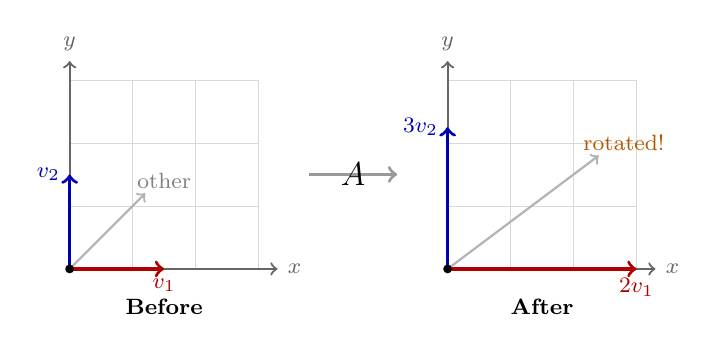
\begin{tikzpicture}[scale=0.8]
    % BEFORE transformation
    \begin{scope}
        \draw[very thin, black!15] (0,0) grid (3,3);
        \draw[->, thick, black!60] (0,0) -- (3.3,0) node[right, font=\footnotesize] {$x$};
        \draw[->, thick, black!60] (0,0) -- (0,3.3) node[above, font=\footnotesize] {$y$};

        % Eigenvectors
        \draw[->, very thick, red!70!black] (0,0) -- (1.5,0);
        \node[red!70!black, font=\footnotesize, below] at (1.5,0) {$\vect{v}_1$};
        \draw[->, very thick, blue!70!black] (0,0) -- (0,1.5);
        \node[blue!70!black, font=\footnotesize, left] at (0,1.5) {$\vect{v}_2$};

        % Non-eigenvector
        \draw[->, thick, gray!60] (0,0) -- (1.2,1.2);
        \node[font=\footnotesize, gray] at (1.5,1.4) {other};

        \fill[black] (0,0) circle (2pt);
        \node[font=\footnotesize\bfseries] at (1.5,-0.6) {Before};
    \end{scope}

    % Arrow
    \draw[->, very thick, black!40] (3.8,1.5) -- (5.2,1.5);
    \node[font=\large] at (4.5,1.5) {$\mat{A}$};

    % AFTER transformation
    \begin{scope}[xshift=6cm]
        \draw[very thin, black!15] (0,0) grid (3,3);
        \draw[->, thick, black!60] (0,0) -- (3.3,0) node[right, font=\footnotesize] {$x$};
        \draw[->, thick, black!60] (0,0) -- (0,3.3) node[above, font=\footnotesize] {$y$};

        % Eigenvectors - stretched but same direction
        \draw[->, very thick, red!70!black] (0,0) -- (3,0);
        \node[red!70!black, font=\footnotesize, below] at (3,0) {$2\vect{v}_1$};
        \draw[->, very thick, blue!70!black] (0,0) -- (0,2.25);
        \node[blue!70!black, font=\footnotesize, left] at (0,2.25) {$3\vect{v}_2$};

        % Non-eigenvector - direction changed!
        \draw[->, thick, gray!60] (0,0) -- (2.4,1.8);
        \node[font=\footnotesize, orange!70!black] at (2.8,2) {rotated!};

        \fill[black] (0,0) circle (2pt);
        \node[font=\footnotesize\bfseries] at (1.5,-0.6) {After};
    \end{scope}
\end{tikzpicture}
\end{center}
\vspace{0.2cm}
\begin{center}
\textit{\footnotesize \textcolor{red!70!black}{Eigenvectors: same direction, just stretched} \quad
\textcolor{gray}{Other vectors: direction changes!}}
\end{center}

\textbf{The Key Insight:} Eigenvectors are the "stable directions" of a matrix. They show you the axes along which the transformation is simplest (just scaling, no rotation).
\end{example}

\begin{intuition}
\textbf{Why should you care? (Besides impressing people at parties)}

Eigenvectors are the ``natural coordinates'' of a transformation. They're the directions where the matrix acts in the simplest possible way---just scaling, no spinning.

Think of it like this: Every matrix has a ``personality.'' Most of the time, that personality is complicated. But eigenvectors reveal the matrix's true nature. They're like a personality test for matrices.

If you're analyzing data and want to understand ``what patterns does this data have?'', you look at eigenvectors. They point toward the most important directions in your data. This is literally how PCA (Principal Component Analysis) works, which is used in everything from face recognition to Netflix recommendations.
\end{intuition}

\subsection{A More Interesting Example}

Let's try a matrix that's not so obvious:
\[
\mat{B} = \begin{bmatrix}
3 & 1 \\
0 & 2
\end{bmatrix}
\]

This one's not diagonal, so the eigenvectors aren't staring us in the face. We'll have to do some detective work!

\textbf{The Mystery:} Which directions stay on the same line after this transformation?

\begin{center}
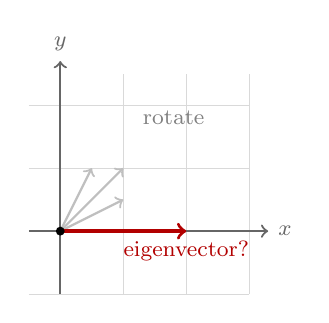
\begin{tikzpicture}[scale=0.8]
    \draw[very thin, black!15] (-0.5,-1) grid (3,2.5);
    \draw[->, thick, black!60] (-0.5,0) -- (3.3,0) node[right, font=\footnotesize] {$x$};
    \draw[->, thick, black!60] (0,-1) -- (0,2.7) node[above, font=\footnotesize] {$y$};

    % Several vectors that rotate
    \draw[->, thick, gray!50] (0,0) -- (1,0.5);
    \draw[->, thick, gray!50] (0,0) -- (1,1);
    \draw[->, thick, gray!50] (0,0) -- (0.5,1);
    \node[gray, font=\footnotesize] at (1.8,1.8) {rotate};

    % Candidate eigenvectors
    \draw[->, very thick, red!70!black] (0,0) -- (2,0);
    \node[red!70!black, font=\footnotesize, below] at (2,0) {eigenvector?};

    \fill[black] (0,0) circle (2pt);
\end{tikzpicture}
\end{center}

\textbf{Claim:} $\vect{v} = [1, 0]$ is an eigenvector.

\textbf{Check:}
\[
\mat{B}\vect{v} = \begin{bmatrix}
3 & 1 \\
0 & 2
\end{bmatrix}
\begin{bmatrix}
1 \\
0
\end{bmatrix}
= \begin{bmatrix}
3 \\
0
\end{bmatrix}
= 3 \begin{bmatrix}
1 \\
0
\end{bmatrix}
= 3\vect{v}
\]

Yes! Eigenvalue is $\lambda_1 = 3$.

\textbf{Claim:} $\vect{w} = [1, -1]$ is an eigenvector.

\textbf{Check:}
\[
\mat{B}\vect{w} = \begin{bmatrix}
3 & 1 \\
0 & 2
\end{bmatrix}
\begin{bmatrix}
1 \\
-1
\end{bmatrix}
= \begin{bmatrix}
3 - 1 \\
0 - 2
\end{bmatrix}
= \begin{bmatrix}
2 \\
-2
\end{bmatrix}
= 2 \begin{bmatrix}
1 \\
-1
\end{bmatrix}
= 2\vect{w}
\]

Yes! Eigenvalue is $\lambda_2 = 2$.

So this matrix has two special directions: $[1, 0]$ (gets scaled by 3) and $[1, -1]$ (gets scaled by 2).

\section{How to Actually Find Eigenvectors (The Recipe)}

\subsection{The Characteristic Equation}

Okay, we've been guessing eigenvectors like we're playing mathematical Wordle. But how do you \textit{actually} find them systematically? Time for some real math!

Here's the strategy. We want to solve:
\[
\mat{A}\vect{v} = \lambda \vect{v}
\]

Rearrange:
\[
\mat{A}\vect{v} - \lambda \vect{v} = \vect{0}
\]

Factor out $\vect{v}$ (careful—we need the identity matrix):
\[
(\mat{A} - \lambda \mat{I})\vect{v} = \vect{0}
\]

For this to have a non-zero solution (we don't want $\vect{v} = \vect{0}$, that's boring), the matrix $(\mat{A} - \lambda\mat{I})$ must be "broken"—it must not have an inverse. Mathematically, its determinant must be zero.

\begin{definition}{The Characteristic Equation}{}
To find eigenvalues of $\mat{A}$, solve:
\[
\det(\mat{A} - \lambda \mat{I}) = 0
\]

This equation (often a polynomial in $\lambda$) is called the \vocab{characteristic equation}. It's the matrix's ``DNA test''---it reveals the eigenvalues hiding inside.

Once you have the eigenvalues $\lambda$, plug each one back into $(\mat{A} - \lambda\mat{I})\vect{v} = \vect{0}$ to find the corresponding eigenvector $\vect{v}$.
\end{definition}

\textbf{Don't panic!} This looks scary, but for 2×2 matrices it's just solving a quadratic equation. You've been doing that since high school. For larger matrices... well, that's why we have computers.

\begin{intuition}
\textbf{Why Does Setting the Determinant to Zero Work?}

Remember from Chapter 1: a matrix has no inverse when its determinant is zero (it squashes space).

The equation $(\mat{A} - \lambda\mat{I})\vect{v} = \vect{0}$ is asking: ``When does this modified matrix send a non-zero vector to zero?''

That can only happen if $(\mat{A} - \lambda\mat{I})$ squashes some direction---i.e., has no inverse---i.e., has determinant zero!

So we're finding the special values of $\lambda$ that ``break'' the matrix $\mat{A} - \lambda\mat{I}$. Those breaking points are exactly the eigenvalues.

\textbf{Analogy:} It's like finding the resonant frequencies of a bridge. At most frequencies, the bridge just vibrates a little. But at certain special frequencies (eigenvalues), it resonates dramatically---small input, huge output. Those are the bridge's ``natural frequencies,'' and they're eigenvalues of the bridge's stiffness matrix!
\end{intuition}

\subsection{Example: Finding Eigenvalues Step by Step}

Let's find the eigenvalues of:
\[
\mat{A} = \begin{bmatrix}
4 & 1 \\
2 & 3
\end{bmatrix}
\]

\textbf{Step 1: Form $\mat{A} - \lambda\mat{I}$}
\[
\mat{A} - \lambda\mat{I} = \begin{bmatrix}
4 & 1 \\
2 & 3
\end{bmatrix}
- \lambda \begin{bmatrix}
1 & 0 \\
0 & 1
\end{bmatrix}
= \begin{bmatrix}
4 - \lambda & 1 \\
2 & 3 - \lambda
\end{bmatrix}
\]

\textbf{Step 2: Compute the determinant}

For a $2 \times 2$ matrix $\begin{bmatrix} a & b \\ c & d \end{bmatrix}$, the determinant is $ad - bc$.

\[
\det(\mat{A} - \lambda\mat{I}) = (4-\lambda)(3-\lambda) - (1)(2)
\]
\[
= 12 - 4\lambda - 3\lambda + \lambda^2 - 2
\]
\[
= \lambda^2 - 7\lambda + 10
\]

\textbf{Step 3: Set it equal to zero and solve}
\[
\lambda^2 - 7\lambda + 10 = 0
\]

Factor (or use quadratic formula):
\[
(\lambda - 5)(\lambda - 2) = 0
\]

So $\lambda_1 = 5$ and $\lambda_2 = 2$. Those are the eigenvalues!

\textbf{Step 4: Find the eigenvectors}

For $\lambda_1 = 5$, solve $(\mat{A} - 5\mat{I})\vect{v} = \vect{0}$:
\[
\begin{bmatrix}
-1 & 1 \\
2 & -2
\end{bmatrix}
\begin{bmatrix}
v_1 \\
v_2
\end{bmatrix}
= \begin{bmatrix}
0 \\
0
\end{bmatrix}
\]

First row: $-v_1 + v_2 = 0 \Rightarrow v_2 = v_1$

So any vector of the form $\begin{bmatrix} v_1 \\ v_1 \end{bmatrix} = v_1 \begin{bmatrix} 1 \\ 1 \end{bmatrix}$ works.

Eigenvector for $\lambda_1 = 5$: $\vect{v}_1 = [1, 1]$ (or any scalar multiple)

For $\lambda_2 = 2$, solve $(\mat{A} - 2\mat{I})\vect{v} = \vect{0}$:
\[
\begin{bmatrix}
2 & 1 \\
2 & 1
\end{bmatrix}
\begin{bmatrix}
v_1 \\
v_2
\end{bmatrix}
= \begin{bmatrix}
0 \\
0
\end{bmatrix}
\]

First row: $2v_1 + v_2 = 0 \Rightarrow v_2 = -2v_1$

Eigenvector for $\lambda_2 = 2$: $\vect{v}_2 = [1, -2]$ (or any scalar multiple)

\textbf{Summary:}
\begin{itemize}
    \item Eigenvalue $\lambda_1 = 5$ with eigenvector $[1, 1]$
    \item Eigenvalue $\lambda_2 = 2$ with eigenvector $[1, -2]$
\end{itemize}

\textbf{Let's Visualize What We Found:}

\begin{center}
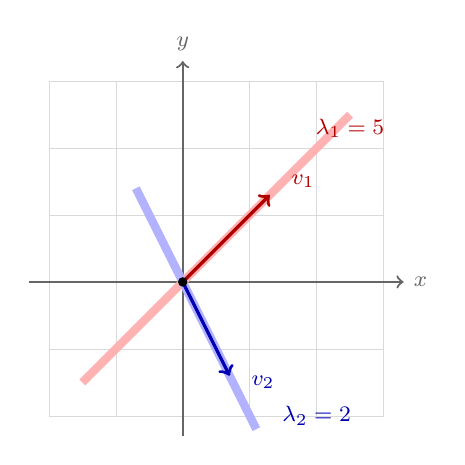
\begin{tikzpicture}[scale=0.85]
    % Grid
    \draw[very thin, black!15] (-2,-2) grid (3,3);

    % Axes
    \draw[->, thick, black!60] (-2.3,0) -- (3.3,0) node[right, font=\footnotesize] {$x$};
    \draw[->, thick, black!60] (0,-2.3) -- (0,3.3) node[above, font=\footnotesize] {$y$};

    % Eigenspace lines (light background)
    \draw[red!30, line width=3pt] (-1.5,-1.5) -- (2.5,2.5);
    \draw[blue!30, line width=3pt] (-0.7,1.4) -- (1.1,-2.2);

    % Eigenvector 1
    \draw[->, very thick, red!70!black] (0,0) -- (1.3,1.3);
    \node[red!70!black, font=\footnotesize] at (1.8,1.5) {$\vect{v}_1$};
    \node[red!70!black, font=\footnotesize] at (2.5,2.3) {$\lambda_1 = 5$};

    % Eigenvector 2
    \draw[->, very thick, blue!70!black] (0,0) -- (0.7,-1.4);
    \node[blue!70!black, font=\footnotesize] at (1.2,-1.5) {$\vect{v}_2$};
    \node[blue!70!black, font=\footnotesize] at (2.0,-2.0) {$\lambda_2 = 2$};

    % Origin
    \fill[black] (0,0) circle (2pt);
\end{tikzpicture}
\end{center}
\vspace{0.1cm}
\begin{center}
\textit{\footnotesize Shaded lines = eigenspaces (all multiples of eigenvectors)}
\end{center}
\vspace{0.2cm}
\textit{The dashed lines show the ``eigenspaces''---the matrix only stretches along these directions!}

\begin{intuition}
\textbf{What did we just do?}

We found the two ``natural directions'' of this matrix. Multiply by $[1, 1]$? Stretches by 5. Multiply by $[1, -2]$? Stretches by 2. Everything else is a cocktail of these two behaviors.

\textbf{Real-world analogy:} Imagine pushing on a wobbly table. Most directions cause it to tip, wobble, and generally misbehave. But there are exactly two special directions where it just slides smoothly without drama. Those are the eigendirections! Every matrix has its own ``drama-free zones.''
\end{intuition}

\begin{intuition}
\textbf{The ``Eigenvalue Decoder Ring''}

Here's a cheat sheet for interpreting eigenvalues in applications:

\begin{center}
\begin{tabular}{ll}
\textbf{Eigenvalue} & \textbf{What it means} \\
\hline
$\lambda > 1$ & Growth/expansion in that direction \\
$\lambda = 1$ & Equilibrium/steady state \\
$0 < \lambda < 1$ & Decay/contraction \\
$\lambda = 0$ & That direction is destroyed \\
$\lambda < 0$ & Oscillation/flipping \\
$|\lambda_1| \gg |\lambda_2|$ & One direction dominates \\
All $|\lambda| < 1$ & System converges to zero \\
Any $|\lambda| > 1$ & System explodes! \\
\end{tabular}
\end{center}

\textbf{In neural networks:} If the eigenvalues of weight matrices have magnitude $>1$, gradients explode during training. If they're all $<1$, gradients vanish. The sweet spot is near 1, which is why careful initialization matters so much!
\end{intuition}

\section{Why Eigenvectors Are Magical}

\subsection{Beautiful Properties}

\begin{theorem}{Cool Facts About Eigenvalues}{}
For a matrix $\mat{A}$:

\textbf{1. Sum of eigenvalues = trace (sum of diagonal elements)}
\[
\lambda_1 + \lambda_2 + \cdots + \lambda_n = a_{11} + a_{22} + \cdots + a_{nn}
\]

\textbf{2. Product of eigenvalues = determinant}
\[
\lambda_1 \times \lambda_2 \times \cdots \times \lambda_n = \det(\mat{A})
\]

\textbf{3. $\mat{A}$ is invertible $\Leftrightarrow$ all eigenvalues are non-zero}

If any $\lambda = 0$, the matrix squashes some direction to zero, so you can't undo it.

\textbf{4. Eigenvectors from different eigenvalues are linearly independent}

They point in genuinely different directions—no redundancy!
\end{theorem}

\begin{example}
For $\mat{A} = \begin{bmatrix} 4 & 1 \\ 2 & 3 \end{bmatrix}$, we found $\lambda_1 = 5, \lambda_2 = 2$.

Check:
\begin{itemize}
    \item Trace: $4 + 3 = 7 = 5 + 2$ (check!)
    \item Determinant: $(4)(3) - (1)(2) = 10 = 5 \times 2$ (check!)
\end{itemize}

These properties give you a quick sanity check when finding eigenvalues!
\end{example}

\subsection{Special Case: Symmetric Matrices Are the Best}

Symmetric matrices are the golden retrievers of the matrix world---friendly, predictable, and everybody loves them.

\begin{theorem}{Spectral Theorem (Simplified)}{}
If $\mat{A}$ is symmetric (i.e., $\mat{A} = \mat{A}^\top$), then:
\begin{itemize}
    \item All eigenvalues are \textbf{real numbers} (no imaginary nonsense!)
    \item Eigenvectors from different eigenvalues are \textbf{perpendicular} (orthogonal)
    \item You can always find $n$ perpendicular eigenvectors for an $n \times n$ symmetric matrix
\end{itemize}
\end{theorem}

\textbf{Why this is AMAZING:} Symmetric matrices are super well-behaved. Their eigenvectors form a nice perpendicular coordinate system, which makes everything cleaner. It's like they went to finishing school.

\begin{intuition}
\textbf{Why Are Symmetric Matrices So Special?}

Here's the deep reason: symmetric matrices represent ``undirected'' relationships.

\begin{itemize}
    \item If person A's influence on person B equals B's influence on A, the influence matrix is symmetric
    \item If the force between particle A and B equals the force between B and A (Newton's third law!), the interaction matrix is symmetric
    \item If the correlation between variables X and Y equals the correlation between Y and X, the correlation matrix is symmetric
\end{itemize}

Nature loves symmetry, and symmetric matrices inherit that beauty. They're honest---they don't have hidden asymmetries that could cause weird complex eigenvalues or non-perpendicular eigenvectors.

\textbf{The Guarantee:} For any $n \times n$ symmetric matrix, you can ALWAYS find $n$ perpendicular eigenvectors that form a complete basis. No exceptions. No edge cases. Mathematics at its most elegant.
\end{intuition}

\begin{connection}
\textbf{Where symmetric matrices show up in AI:}

\begin{itemize}
    \item \textbf{Covariance matrices} (measure how data dimensions correlate) are always symmetric
    \item \textbf{Graph adjacency matrices} (social networks, molecule structures) are often symmetric
    \item \textbf{Hessian matrices} (second derivatives in optimization) are symmetric
    \item \textbf{Kernel matrices} (in SVMs and Gaussian processes) are symmetric positive semi-definite
    \item \textbf{Gram matrices} ($\mat{X}^\top\mat{X}$, used everywhere) are always symmetric
\end{itemize}

So eigenvectors of symmetric matrices are everywhere in machine learning!
\end{connection}

\begin{example}
\textbf{Google's PageRank: The Billion-Dollar Eigenvector}

Here's a real story about eigenvectors making history.

In 1998, Larry Page and Sergey Brin had a problem: how do you rank web pages by importance? Their insight: a page is important if important pages link to it. But that's circular!

The solution: model the web as a matrix. Entry $(i,j)$ represents the probability of clicking from page $j$ to page $i$. The ``importance'' vector $\vect{r}$ should satisfy:
\[
\mat{A}\vect{r} = \vect{r}
\]

Wait... that's an eigenvector equation with $\lambda = 1$!

The importance ranking of every webpage is literally the eigenvector of the web's link matrix with eigenvalue 1. Google's original algorithm was just finding an eigenvector.

\textbf{The punchline:} The eigenvector that launched a trillion-dollar company. Linear algebra pays.
\end{example}

\section{Eigendecomposition: Breaking Matrices Apart}

\subsection{The Big Idea}

If a matrix has $n$ linearly independent eigenvectors, we can "decompose" it into simpler pieces.

\begin{definition}{Eigendecomposition}{}
If $\mat{A}$ has $n$ linearly independent eigenvectors $\vect{v}_1, \ldots, \vect{v}_n$ with eigenvalues $\lambda_1, \ldots, \lambda_n$, then:
\[
\mat{A} = \mat{V} \mat{\Lambda} \mat{V}^{-1}
\]

where:
\begin{itemize}
    \item $\mat{V} = [\vect{v}_1 \, | \, \vect{v}_2 \, | \, \cdots \, | \, \vect{v}_n]$ (columns are eigenvectors)
    \item $\mat{\Lambda} = \begin{bmatrix} \lambda_1 & 0 & \cdots & 0 \\ 0 & \lambda_2 & \cdots & 0 \\ \vdots & \vdots & \ddots & \vdots \\ 0 & 0 & \cdots & \lambda_n \end{bmatrix}$ (diagonal matrix of eigenvalues)
\end{itemize}
\end{definition}

\textbf{In plain English:} "Any nice matrix is just a rotation ($\mat{V}^{-1}$), a stretch along axes ($\mat{\Lambda}$), and a rotation back ($\mat{V}$)."

\begin{intuition}
Think of $\mat{A}$ as a complicated transformation. The eigendecomposition says:

\textbf{Step 1:} Rotate to the eigenvector coordinate system ($\mat{V}^{-1}$)

\textbf{Step 2:} In this new system, just scale each axis independently ($\mat{\Lambda}$)—super simple!

\textbf{Step 3:} Rotate back to the original coordinates ($\mat{V}$)

It's like saying "this complex motion is just a simple stretch, if you look at it from the right angle."

\textbf{VISUALIZING EIGENDECOMPOSITION: The Three-Step Dance}

Think of it as a change of clothes: go to your ``eigen-closet,'' do the simple scaling, then change back.

\vspace{0.3cm}
\begin{center}
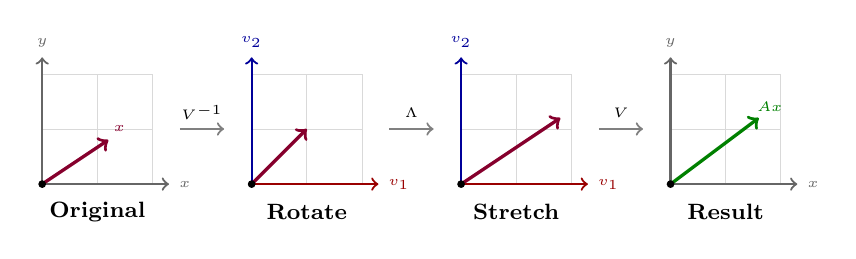
\begin{tikzpicture}[scale=0.7]
    % Step 1: Original
    \begin{scope}
        \draw[very thin, black!15] (0,0) grid (2,2);
        \draw[->, thick, black!60] (0,0) -- (2.3,0) node[right, font=\tiny] {$x$};
        \draw[->, thick, black!60] (0,0) -- (0,2.3) node[above, font=\tiny] {$y$};
        \draw[->, very thick, purple!70!black] (0,0) -- (1.2,0.8);
        \node[purple!70!black, font=\tiny] at (1.4,1) {$\vect{x}$};
        \fill[black] (0,0) circle (2pt);
        \node[font=\footnotesize\bfseries] at (1,-0.5) {Original};
    \end{scope}

    % Arrow 1
    \draw[->, thick, black!50] (2.5,1) -- (3.3,1);
    \node[font=\tiny] at (2.9,1.3) {$\mat{V}^{-1}$};

    % Step 2: Eigen-basis
    \begin{scope}[xshift=3.8cm]
        \draw[very thin, black!15] (0,0) grid (2,2);
        \draw[->, thick, red!60!black] (0,0) -- (2.3,0) node[right, font=\tiny] {$\vect{v}_1$};
        \draw[->, thick, blue!60!black] (0,0) -- (0,2.3) node[above, font=\tiny] {$\vect{v}_2$};
        \draw[->, very thick, purple!70!black] (0,0) -- (1,1);
        \fill[black] (0,0) circle (2pt);
        \node[font=\footnotesize\bfseries] at (1,-0.5) {Rotate};
    \end{scope}

    % Arrow 2
    \draw[->, thick, black!50] (6.3,1) -- (7.1,1);
    \node[font=\tiny] at (6.7,1.3) {$\mat{\Lambda}$};

    % Step 3: Stretch
    \begin{scope}[xshift=7.6cm]
        \draw[very thin, black!15] (0,0) grid (2,2);
        \draw[->, thick, red!60!black] (0,0) -- (2.3,0) node[right, font=\tiny] {$\vect{v}_1$};
        \draw[->, thick, blue!60!black] (0,0) -- (0,2.3) node[above, font=\tiny] {$\vect{v}_2$};
        \draw[->, very thick, purple!70!black] (0,0) -- (1.8,1.2);
        \fill[black] (0,0) circle (2pt);
        \node[font=\footnotesize\bfseries] at (1,-0.5) {Stretch};
    \end{scope}

    % Arrow 3
    \draw[->, thick, black!50] (10.1,1) -- (10.9,1);
    \node[font=\tiny] at (10.5,1.3) {$\mat{V}$};

    % Step 4: Result
    \begin{scope}[xshift=11.4cm]
        \draw[very thin, black!15] (0,0) grid (2,2);
        \draw[->, thick, black!60] (0,0) -- (2.3,0) node[right, font=\tiny] {$x$};
        \draw[->, thick, black!60] (0,0) -- (0,2.3) node[above, font=\tiny] {$y$};
        \draw[->, very thick, green!50!black] (0,0) -- (1.6,1.2);
        \node[green!50!black, font=\tiny] at (1.8,1.4) {$\mat{A}\vect{x}$};
        \fill[black] (0,0) circle (2pt);
        \node[font=\footnotesize\bfseries] at (1,-0.5) {Result};
    \end{scope}
\end{tikzpicture}
\end{center}
\vspace{0.2cm}

\textbf{The Beautiful Insight:} In the eigenvector coordinate system, the transformation is just diagonal scaling! All the complexity comes from rotating in and out of that special coordinate system.

\textbf{Analogy:} Imagine trying to describe a spiral staircase. In normal coordinates, it's complicated. But if you use cylindrical coordinates (angle, radius, height), it's just "go up while staying at constant radius"—much simpler! Eigendecomposition finds those simpler coordinates.
\end{intuition}

\begin{example}
\textbf{Eigendecomposition in Action}

Let's actually decompose a matrix. Take:
\[
\mat{A} = \begin{bmatrix} 2 & 1 \\ 1 & 2 \end{bmatrix}
\]

\textbf{Step 1: Find eigenvalues}

$\det(\mat{A} - \lambda\mat{I}) = (2-\lambda)^2 - 1 = \lambda^2 - 4\lambda + 3 = (\lambda-3)(\lambda-1) = 0$

So $\lambda_1 = 3$ and $\lambda_2 = 1$.

\textbf{Step 2: Find eigenvectors}

For $\lambda_1 = 3$: Solve $(\mat{A} - 3\mat{I})\vect{v} = 0$
\[
\begin{bmatrix} -1 & 1 \\ 1 & -1 \end{bmatrix}\vect{v} = 0 \Rightarrow \vect{v}_1 = \begin{bmatrix} 1 \\ 1 \end{bmatrix}
\]

For $\lambda_2 = 1$: Solve $(\mat{A} - \mat{I})\vect{v} = 0$
\[
\begin{bmatrix} 1 & 1 \\ 1 & 1 \end{bmatrix}\vect{v} = 0 \Rightarrow \vect{v}_2 = \begin{bmatrix} 1 \\ -1 \end{bmatrix}
\]

\textbf{Step 3: Assemble the decomposition}

Normalize (make length 1): $\hat{\vect{v}}_1 = \frac{1}{\sqrt{2}}[1,1]^\top$, $\hat{\vect{v}}_2 = \frac{1}{\sqrt{2}}[1,-1]^\top$

Since $\mat{A}$ is symmetric, $\mat{V}$ is orthogonal, so $\mat{V}^{-1} = \mat{V}^\top$:
\[
\mat{A} = \mat{V}\mat{\Lambda}\mat{V}^\top = \frac{1}{2}\begin{bmatrix} 1 & 1 \\ 1 & -1 \end{bmatrix} \begin{bmatrix} 3 & 0 \\ 0 & 1 \end{bmatrix} \begin{bmatrix} 1 & 1 \\ 1 & -1 \end{bmatrix}
\]

\textbf{Interpretation:} This matrix stretches by 3 along the diagonal $[1,1]$ and by 1 along the anti-diagonal $[1,-1]$. That's it! The symmetric matrix was secretly just doing axis-aligned stretching in a rotated coordinate system.
\end{example}

\subsection{Why This Is Insanely Useful}

\textbf{1. Computing matrix powers:}

If you need to compute $\mat{A}^{100}$ (multiply $\mat{A}$ by itself 100 times), it's hard. But with eigendecomposition:
\[
\mat{A}^{100} = (\mat{V}\mat{\Lambda}\mat{V}^{-1})^{100} = \mat{V}\mat{\Lambda}^{100}\mat{V}^{-1}
\]

And $\mat{\Lambda}^{100}$ is easy—just raise each eigenvalue to the 100th power:
\[
\mat{\Lambda}^{100} = \begin{bmatrix}
\lambda_1^{100} & 0 & \cdots \\
0 & \lambda_2^{100} & \cdots \\
\vdots & \vdots & \ddots
\end{bmatrix}
\]

\textbf{2. Understanding long-term behavior:}

If you repeatedly apply $\mat{A}$ to a vector (like in iterative algorithms), the behavior is dominated by the largest eigenvalue. This tells you if things converge, diverge, or oscillate.

\textbf{3. Principal Component Analysis (PCA):}

PCA finds the directions of maximum variance in data. How? By finding the eigenvectors of the covariance matrix! The eigenvector with the largest eigenvalue points in the direction where data varies the most.

\begin{intuition}
\textbf{PCA: Finding the ``Soul'' of Your Data}

Imagine you have data about people: height, weight, shoe size, arm length, etc. That's maybe 10 dimensions. Hard to visualize!

PCA asks: ``What are the REAL underlying factors?'' Maybe all those measurements are really driven by just 2-3 underlying factors (like overall body size, body proportions, etc.).

\textbf{The Algorithm:}
\begin{enumerate}
    \item Compute the covariance matrix of your data
    \item Find its eigenvectors and eigenvalues
    \item The eigenvector with the LARGEST eigenvalue = the direction of most variance = the most important ``factor''
    \item The second largest = second most important, perpendicular to the first
    \item Keep the top $k$ eigenvectors, discard the rest
\end{enumerate}

You've now reduced 10 dimensions to $k$ dimensions, keeping the most important patterns!

\textbf{Real example:} In face recognition, faces are ~10,000 pixels. PCA finds that most face variation can be captured by ~100 ``eigenfaces'' (eigenvectors of the face covariance matrix). 100× compression while keeping what matters!
\end{intuition}

\textbf{Visual Example of Matrix Powers:}

\vspace{0.2cm}
\begin{center}
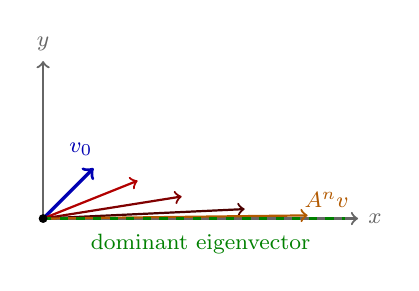
\begin{tikzpicture}[scale=0.8]
    % Axes
    \draw[->, thick, black!60] (0,0) -- (5,0) node[right, font=\footnotesize] {$x$};
    \draw[->, thick, black!60] (0,0) -- (0,2.5) node[above, font=\footnotesize] {$y$};

    % Initial vector
    \draw[->, very thick, blue!70!black] (0,0) -- (0.8,0.8);
    \node[blue!70!black, font=\footnotesize] at (0.6,1.1) {$\vect{v}_0$};

    % After repeated multiplication - converging to dominant eigenvector
    \draw[->, thick, red!70!black] (0,0) -- (1.5,0.6);
    \draw[->, thick, red!50!black] (0,0) -- (2.2,0.35);
    \draw[->, thick, red!30!black] (0,0) -- (3.2,0.15);
    \draw[->, thick, orange!70!black] (0,0) -- (4.2,0.05);
    \node[orange!70!black, font=\footnotesize] at (4.5,0.3) {$\mat{A}^n\vect{v}$};

    % Dominant eigenvector direction
    \draw[dashed, thick, green!50!black] (0,0) -- (4.8,0);
    \node[green!50!black, font=\footnotesize] at (2.5,-0.4) {dominant eigenvector};

    \fill[black] (0,0) circle (2pt);
\end{tikzpicture}
\end{center}
\vspace{0.1cm}
\begin{center}
\textit{\footnotesize Keep multiplying $\rightarrow$ converge to dominant eigenvector direction!}
\end{center}
\vspace{0.2cm}

\begin{connection}
\textbf{How neural networks use eigendecomposition:}

\begin{itemize}
    \item \textbf{Analyzing training dynamics:} The eigenvalues of the Hessian (matrix of second derivatives) tell you if optimization will be fast or slow. If eigenvalues vary wildly (some huge, some tiny), training is difficult---you need different step sizes for different directions!
    \item \textbf{Compression:} Keep only the eigenvectors with large eigenvalues, discard the rest (dimensionality reduction)
    \item \textbf{Initialization:} Understanding eigenvalues helps design better ways to initialize network weights. Xavier and He initialization are designed to keep eigenvalues near 1.
    \item \textbf{Spectral normalization:} Divide weight matrices by their largest eigenvalue to stabilize GAN training
\end{itemize}
\end{connection}

\begin{intuition}
\textbf{The ``Condition Number'' Problem}

The ratio of the largest to smallest eigenvalue is called the \vocab{condition number}:
\[
\kappa(\mat{A}) = \frac{|\lambda_{\max}|}{|\lambda_{\min}|}
\]

\begin{itemize}
    \item $\kappa \approx 1$: Well-conditioned. All directions are treated similarly. Easy to work with!
    \item $\kappa \gg 1$: Ill-conditioned. Some directions are amplified WAY more than others. Numerically unstable!
\end{itemize}

\textbf{In optimization:} If the Hessian has $\kappa = 1000$, gradient descent struggles. It takes tiny steps in some directions and huge steps in others. That's why we use adaptive optimizers like Adam---they effectively rescale to make the condition number closer to 1.

\textbf{Analogy:} Optimizing with high condition number is like walking through a steep, narrow valley. You keep bouncing off the walls instead of going down. Better to transform the valley into a nice bowl first!
\end{intuition}

\section{Singular Value Decomposition (SVD): The Ultimate Weapon}

\subsection{What If the Matrix Isn't Square?}

Eigendecomposition is great, but it has a fatal flaw: it only works for square matrices. What about $m \times n$ matrices (different numbers of rows and columns)? What about matrices that don't play nice with eigenvectors?

Enter SVD: the most powerful matrix decomposition of all time. If eigendecomposition is a Swiss Army knife, SVD is the entire hardware store. It works on \textit{any} matrix. Any size. Any shape. No exceptions.

\begin{intuition}
\textbf{SVD vs Eigendecomposition: The Key Difference}

\textbf{Eigendecomposition} asks: ``What directions does this matrix leave unchanged (except for scaling)?''
\begin{itemize}
    \item Only works for square matrices
    \item Might not find enough eigenvectors
    \item Input and output are in the same space
\end{itemize}

\textbf{SVD} asks: ``What are the best input directions that map to the best output directions?''
\begin{itemize}
    \item Works for ANY matrix (any shape!)
    \item Always finds a complete set of directions
    \item Input and output can be different spaces
\end{itemize}

\textbf{Analogy:} Eigendecomposition is like finding the natural vibration modes of a single drum. SVD is like finding the best way to transmit sound from a speaker (input space) to a microphone (output space)---even if they're in different rooms!
\end{intuition}

\textbf{Quick Setup:} Imagine you have a rectangular matrix (like a transformation that changes dimensions—3D to 2D, or 100D to 50D). How do you understand what it does?

\begin{definition}{Singular Value Decomposition}{}
\textbf{Any} matrix $\mat{A} \in \R^{m \times n}$ can be decomposed as:
\[
\mat{A} = \mat{U} \mat{\Sigma} \mat{V}^\top
\]

where:
\begin{itemize}
    \item $\mat{U} \in \R^{m \times m}$ is orthogonal (columns are perpendicular unit vectors)
    \item $\mat{\Sigma} \in \R^{m \times n}$ is diagonal (only has entries on the main diagonal)
    \item $\mat{V} \in \R^{n \times n}$ is orthogonal
    \item The diagonal entries $\sigma_1 \geq \sigma_2 \geq \cdots \geq 0$ are called \vocab{singular values}
\end{itemize}
\end{definition}

In plain English: "Every matrix is just a rotation, a stretch along perpendicular axes, and another rotation."

\textbf{THE SVD TRANSFORMATION: Circle to Ellipse}

The beautiful thing about SVD: it shows that \textit{every} matrix turns a circle into an ellipse. That's it! Rotate, stretch into ellipse, rotate again.

\vspace{0.2cm}
\begin{center}
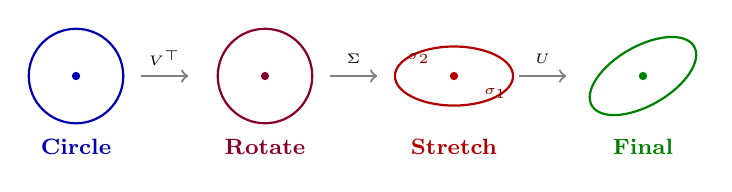
\begin{tikzpicture}[scale=0.75]
    % Step 1: Unit circle
    \begin{scope}
        \draw[thick, blue!70!black] (1,1) circle (0.8);
        \fill[blue!70!black] (1,1) circle (2pt);
        \node[font=\footnotesize\bfseries, blue!70!black] at (1,-0.2) {Circle};
    \end{scope}

    % Arrow 1
    \draw[->, thick, black!50] (2.1,1) -- (2.9,1);
    \node[font=\tiny] at (2.5,1.3) {$\mat{V}^\top$};

    % Step 2: Rotated circle
    \begin{scope}[xshift=3.2cm]
        \draw[thick, purple!70!black] (1,1) circle (0.8);
        \fill[purple!70!black] (1,1) circle (2pt);
        \node[font=\footnotesize\bfseries, purple!70!black] at (1,-0.2) {Rotate};
    \end{scope}

    % Arrow 2
    \draw[->, thick, black!50] (5.3,1) -- (6.1,1);
    \node[font=\tiny] at (5.7,1.3) {$\mat{\Sigma}$};

    % Step 3: Ellipse (stretched)
    \begin{scope}[xshift=6.4cm]
        \draw[thick, red!70!black] (1,1) ellipse (1cm and 0.5cm);
        \fill[red!70!black] (1,1) circle (2pt);
        \node[font=\footnotesize\bfseries, red!70!black] at (1,-0.2) {Stretch};
        \node[font=\tiny, red!50!black] at (1.7,0.7) {$\sigma_1$};
        \node[font=\tiny, red!50!black] at (0.4,1.3) {$\sigma_2$};
    \end{scope}

    % Arrow 3
    \draw[->, thick, black!50] (8.5,1) -- (9.3,1);
    \node[font=\tiny] at (8.9,1.3) {$\mat{U}$};

    % Step 4: Rotated ellipse
    \begin{scope}[xshift=9.6cm]
        \draw[thick, green!50!black, rotate around={30:(1,1)}] (1,1) ellipse (1cm and 0.5cm);
        \fill[green!50!black] (1,1) circle (2pt);
        \node[font=\footnotesize\bfseries, green!50!black] at (1,-0.2) {Final};
    \end{scope}
\end{tikzpicture}
\end{center}
\vspace{0.1cm}
\begin{center}
\textit{\footnotesize Every matrix turns a circle into an ellipse: Rotate $\rightarrow$ Stretch $\rightarrow$ Rotate}
\end{center}
\vspace{0.2cm}

\textbf{What Just Happened:}
\begin{enumerate}
    \item Started with unit circle (all possible inputs of length 1)
    \item $\mat{V}^\top$: Rotated to the "right" input coordinate system
    \item $\mat{\Sigma}$: Stretched along perpendicular axes (circle → ellipse)
    \item $\mat{U}$: Rotated to the "right" output coordinate system
    \item Result: An ellipse! The matrix turned a circle into an ellipse!
\end{enumerate}

\textbf{The Singular Values:} The entries in $\mat{\Sigma}$ (the $\sigma_i$ values) are how much stretching happens along each axis. They're called "singular values."

\textbf{Key facts about singular values:}
\begin{itemize}
    \item Always real and non-negative (unlike eigenvalues, which can be complex or negative)
    \item Always ordered: $\sigma_1 \geq \sigma_2 \geq \cdots \geq \sigma_r > 0$
    \item The number of non-zero singular values = the rank of the matrix
    \item $\sigma_1$ is the maximum ``stretching factor'' of the matrix
    \item $\sigma_r$ (smallest non-zero) is the minimum stretching factor
    \item Their ratio $\sigma_1/\sigma_r$ is the condition number!
\end{itemize}

\begin{intuition}
\textbf{Think of SVD like this:}

You have a transformation $\mat{A}$ that might stretch, rotate, skew, project—do all kinds of crazy stuff.

SVD says: "Actually, if you pick the RIGHT input coordinate system ($\mat{V}^\top$) and the RIGHT output coordinate system ($\mat{U}$), then $\mat{A}$ is just stretching/shrinking along perpendicular directions ($\mat{\Sigma}$). No rotation, no weird stuff."

It's finding the "natural coordinates" for both input and output spaces.

\textbf{The Deep Connection to Eigendecomposition:}

Here's a beautiful fact: the singular values of $\mat{A}$ are the square roots of the eigenvalues of $\mat{A}^\top\mat{A}$ (or $\mat{A}\mat{A}^\top$).

Why? Because $\mat{A}^\top\mat{A}$ is symmetric (always!), so it has nice real eigenvalues. And:
\[
\mat{A}^\top\mat{A} = (\mat{U}\mat{\Sigma}\mat{V}^\top)^\top(\mat{U}\mat{\Sigma}\mat{V}^\top) = \mat{V}\mat{\Sigma}^\top\mat{U}^\top\mat{U}\mat{\Sigma}\mat{V}^\top = \mat{V}\mat{\Sigma}^2\mat{V}^\top
\]

So the right singular vectors ($\mat{V}$) are eigenvectors of $\mat{A}^\top\mat{A}$, and the singular values squared are the eigenvalues!

This is often how SVD is computed in practice: find the eigendecomposition of $\mat{A}^\top\mat{A}$, then take square roots.
\end{intuition}

\subsection{Why SVD Is the Swiss Army Knife of Linear Algebra}

SVD can do EVERYTHING:

\textbf{1. Solve linear systems:} Even overdetermined or underdetermined ones

\textbf{2. Find the rank:} Count how many singular values are non-zero

\textbf{3. Compress data:} Keep only the largest singular values

\textbf{4. Denoise data:} Small singular values = noise; drop them

\textbf{5. Pseudoinverse:} Invert non-square or singular matrices

\textbf{6. Recommendation systems:} Collaborative filtering (Netflix prize!)

\textbf{7. Latent semantic analysis:} Discover hidden topics in text

\textbf{8. Face recognition:} Eigenfaces are really singular vectors

\textbf{9. Calculate matrix norms:} $\|\mat{A}\|_2 = \sigma_1$ (largest singular value)

\textbf{10. Low-rank approximation:} Best possible compression (Eckart-Young theorem)

\begin{theorem}{Eckart-Young Theorem (The Best Compression Guarantee)}{}
The best rank-$k$ approximation to a matrix $\mat{A}$ (in terms of minimizing the Frobenius norm of the error) is given by truncated SVD:
\[
\mat{A}_k = \sum_{i=1}^{k} \sigma_i \vect{u}_i \vect{v}_i^\top
\]

No other rank-$k$ matrix is closer to $\mat{A}$. SVD gives you the optimal compression, guaranteed!
\end{theorem}

\subsection{Example: Image Compression with SVD}

Here's something mind-blowingly practical: an image is just a matrix of pixel brightnesses. Every photo you've ever taken is secretly a matrix. And SVD can compress it like a boss!

\textbf{The Idea:}
\[
\mat{A} = \mat{U}\mat{\Sigma}\mat{V}^\top = \sigma_1 \vect{u}_1 \vect{v}_1^\top + \sigma_2 \vect{u}_2 \vect{v}_2^\top + \cdots + \sigma_r \vect{u}_r \vect{v}_r^\top
\]

This is a sum of rank-1 matrices, each scaled by $\sigma_i$.

\textbf{Compression trick:} Keep only the largest $k$ terms:
\[
\mat{A}_{\text{compressed}} \approx \sigma_1 \vect{u}_1 \vect{v}_1^\top + \cdots + \sigma_k \vect{u}_k \vect{v}_k^\top
\]

If $k$ is much smaller than the full rank, you've compressed the image! You're storing way fewer numbers, and the image still looks good because the large singular values capture most of the information.

\textbf{Real numbers:} A 1000×1000 image has 1,000,000 pixels. With rank-50 SVD, you store only about 100,000 numbers---10× compression! And it usually looks almost identical. This is basically how JPEG works (with some extra tricks).

\begin{intuition}
\textbf{Why Does This Work? The ``Energy'' Interpretation}

The singular values tell you how much ``energy'' or ``importance'' is in each direction. For most real-world data:
\begin{itemize}
    \item The first few singular values are HUGE (capture main patterns)
    \item The rest decay rapidly (capture noise and fine details)
\end{itemize}

\begin{center}
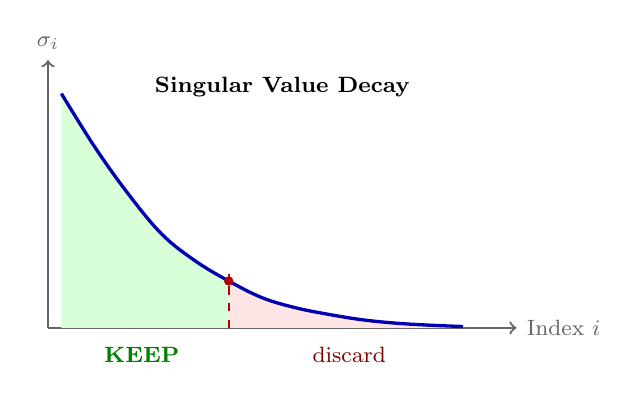
\begin{tikzpicture}[scale=0.85]
    % Axes
    \draw[->, thick, black!60] (0,0) -- (7,0) node[right, font=\footnotesize] {Index $i$};
    \draw[->, thick, black!60] (0,0) -- (0,4) node[above, font=\footnotesize] {$\sigma_i$};

    % Keep region (green)
    \fill[green!15] (0.2,0) -- (0.2,3.5) -- (0.7,2.7) -- (1.2,2.0) -- (1.7,1.4) -- (2.2,1.0) -- (2.7,0.7) -- (2.7,0) -- cycle;

    % Discard region (red)
    \fill[red!10] (2.7,0) -- (2.7,0.7) -- (3.2,0.45) -- (3.7,0.3) -- (4.2,0.2) -- (4.7,0.12) -- (5.2,0.07) -- (5.7,0.04) -- (6.2,0.02) -- (6.2,0) -- cycle;

    % Decay curve
    \draw[blue!70!black, very thick]
        plot[smooth, tension=0.6] coordinates {(0.2,3.5) (0.7,2.7) (1.2,2.0) (1.7,1.4) (2.2,1.0) (2.7,0.7) (3.2,0.45) (3.7,0.3) (4.2,0.2) (4.7,0.12) (5.2,0.07) (5.7,0.04) (6.2,0.02)};

    % Cutoff line
    \draw[dashed, red!70!black, thick] (2.7,0) -- (2.7,0.8);
    \fill[red!70!black] (2.7,0.7) circle (2pt);

    % Labels
    \node[green!50!black, font=\footnotesize\bfseries] at (1.4,-0.4) {KEEP};
    \node[red!50!black, font=\footnotesize] at (4.5,-0.4) {discard};

    \node[font=\footnotesize\bfseries] at (3.5,3.6) {Singular Value Decay};
\end{tikzpicture}
\end{center}

When you keep only the top $k$ singular values, you're keeping the ``important'' patterns and discarding the noise. The retained energy is:
\[
\text{Energy retained} = \frac{\sigma_1^2 + \cdots + \sigma_k^2}{\sigma_1^2 + \cdots + \sigma_n^2}
\]

Often, 95\%+ of the energy is in the first 10\% of singular values!
\end{intuition}

\begin{connection}
\textbf{SVD in LLMs:}

\begin{itemize}
    \item \textbf{LoRA (Low-Rank Adaptation):} Instead of fine-tuning a full weight matrix, LoRA learns a low-rank update $\mat{A} + \mat{U}\mat{V}^\top$ where $\mat{U}$ and $\mat{V}$ are skinny matrices. This is basically SVD thinking!

    \item \textbf{Latent Semantic Analysis:} Early NLP technique that used SVD on word-document matrices to discover topics

    \item \textbf{Analyzing attention patterns:} SVD can decompose attention matrices to understand what the model is focusing on
\end{itemize}

Modern compression techniques for LLMs (quantization, pruning, distillation) are often inspired by SVD ideas: "keep the important directions, discard the rest."
\end{connection}

\begin{example}
\textbf{LoRA: The SVD-Inspired Revolution in Fine-Tuning}

A GPT-3 sized model has ~175 billion parameters. Fine-tuning ALL of them for your specific task is:
\begin{itemize}
    \item Computationally expensive (need huge GPUs)
    \item Memory-intensive (need to store gradients for 175B parameters)
    \item Risky (might forget what it learned before)
\end{itemize}

\textbf{LoRA's insight:} The CHANGE in weights during fine-tuning is probably low-rank! You don't need to change everything---just a few important directions.

Instead of learning a new weight matrix $\mat{W}'$, LoRA learns:
\[
\mat{W}' = \mat{W} + \mat{B}\mat{A}
\]

where $\mat{B}$ is $d \times r$ and $\mat{A}$ is $r \times d$, with $r \ll d$ (e.g., $r = 8$ when $d = 4096$).

\textbf{The math:} $\mat{B}\mat{A}$ is a rank-$r$ matrix. It's like we're only updating in $r$ directions, not all $d$!

\textbf{The savings:} Instead of $d^2$ parameters, we only train $2dr$ parameters. For $d = 4096$ and $r = 8$:
\begin{itemize}
    \item Full fine-tuning: 16,777,216 parameters per layer
    \item LoRA: 65,536 parameters per layer
    \item That's 256× fewer parameters!
\end{itemize}

This is why you can fine-tune LLMs on a laptop now. Thank SVD thinking!
\end{example}

\section{Putting It All Together}

You made it! You now know more about matrices than 99\% of the population. Let's summarize your new superpowers.

\subsection{The Hierarchy of Matrix Decompositions}

\begin{itemize}
    \item \textbf{Eigendecomposition:} Works for square matrices with enough independent eigenvectors
    \begin{itemize}
        \item Best for: Understanding dynamics, computing powers, PCA
        \item Special case: Symmetric matrices have perpendicular eigenvectors
    \end{itemize}

    \item \textbf{SVD:} Works for ANY matrix (square or rectangular)
    \begin{itemize}
        \item Best for: Compression, rank finding, solving systems, recommendation
        \item Always gives perpendicular bases for input and output
    \end{itemize}
\end{itemize}

\subsection{The Big Picture}

All of these decompositions are about the same fundamental idea:

\textbf{"Find the natural coordinate system where the transformation is simplest."}

\begin{itemize}
    \item Eigenvectors: The directions where $\mat{A}$ just scales
    \item SVD: The input/output bases where $\mat{A}$ is just diagonal scaling
\end{itemize}

This philosophy—"find the right coordinates to make things simple"—is central to all of machine learning.

\begin{intuition}
\textbf{The Zen of Matrix Decomposition}

Every matrix decomposition is answering a question:

\begin{center}
\small
\begin{tabular}{lp{6cm}}
\textbf{Decomposition} & \textbf{Question it answers} \\
\hline
Eigendecomposition & What are the natural directions? \\
SVD & What's the best low-rank approximation? \\
LU decomposition & How do I solve linear systems? \\
QR decomposition & How do I find orthogonal bases? \\
Cholesky & How do I factor symmetric PD matrices? \\
\end{tabular}
\end{center}

Each decomposition reveals a different aspect of the matrix's ``personality.'' Learning when to use which is part of becoming a linear algebra master.

\textbf{The Master Skill:} Look at a problem and ask ``What structure can I exploit?'' Is the matrix symmetric? Use eigendecomposition. Need to compress? Use SVD. Solving many systems with the same matrix? Use LU. The right decomposition turns a hard problem into an easy one.
\end{intuition}

\section{Practice Problems}

\begin{intuition}
\textbf{How to Approach These Problems}

Eigenvector problems can feel abstract. Here's a mindset that helps:

\begin{enumerate}
    \item \textbf{Geometric thinking first:} Before computing, ask ``What does this matrix DO?'' Does it stretch? Rotate? Project?
    \item \textbf{Sanity checks:} After finding eigenvalues, verify that trace = sum and determinant = product
    \item \textbf{Interpret your answer:} Don't just compute $\lambda = 3$---think ``this direction gets stretched by 3x''
\end{enumerate}
\end{intuition}

\subsection{Problem 1: Basic Eigenvalues}

Find the eigenvalues and eigenvectors of:
\[
\mat{A} = \begin{bmatrix}
3 & 1 \\
0 & 2
\end{bmatrix}
\]

\textit{Hint: This is an upper triangular matrix. What's special about eigenvalues of triangular matrices?}

\subsection{Problem 2: Eigenvalue Properties}

Given a matrix with eigenvalues $\lambda_1 = 3$, $\lambda_2 = -2$, $\lambda_3 = 5$:
\begin{enumerate}
    \item What is the trace of the matrix?
    \item What is the determinant?
    \item Is the matrix invertible? Why or why not?
\end{enumerate}

\subsection{Problem 3: Understanding Eigenvectors (The Fun One)}

If $\vect{v}$ is an eigenvector of $\mat{A}$ with eigenvalue $\lambda = 2$:
\begin{enumerate}
    \item What is $\mat{A}^{10}\vect{v}$? (Express in terms of $\vect{v}$)
    \item If $\lambda = 0.5$, what happens to $\vect{v}$ as you repeatedly apply $\mat{A}$? Where does it end up?
    \item If $\lambda = -1$, what happens? (Hint: think about $\mat{A}^1\vect{v}$, $\mat{A}^2\vect{v}$, $\mat{A}^3\vect{v}$...)
    \item If $\lambda = 1$, what's special about $\vect{v}$?
    \item \textbf{Challenge:} If a matrix has eigenvalues $\lambda_1 = 1.01$ and $\lambda_2 = 0.99$, what happens to a random vector after applying the matrix 1000 times?
\end{enumerate}

\subsection{Problem 4: Connection to LLMs}

Explain in your own words:
\begin{enumerate}
    \item Why might we want to find the eigenvectors of a word embedding covariance matrix?
    \item How does SVD help compress neural network weights?
    \item What does it mean if an attention matrix has one very large eigenvalue and many small ones?
    \item In LoRA, we approximate weight updates as $\Delta\mat{W} = \mat{B}\mat{A}$ where $\mat{B}$ is $d \times r$ and $\mat{A}$ is $r \times d$. What is the rank of $\Delta\mat{W}$? Why does this save memory?
\end{enumerate}

\subsection{Problem 5: SVD Compression}

A grayscale image is stored as a $100 \times 100$ matrix (10,000 pixels).

\begin{enumerate}
    \item If you compute the full SVD, how many singular values will there be (at most)?
    \item If you keep only the top 10 singular values, how many numbers do you need to store? (Count entries in truncated $\mat{U}$, $\mat{\Sigma}$, and $\mat{V}$)
    \item What is the compression ratio?
    \item If the singular values are $\sigma_1 = 100, \sigma_2 = 50, \sigma_3 = 25, \sigma_4 = 12, \sigma_5 = 6$, and the rest are below 1, what percentage of the ``energy'' ($\sum \sigma_i^2$) is captured by the top 5 components?
\end{enumerate}

\subsection{Problem 6: Geometric Intuition}

Without computing, predict the eigenvectors and eigenvalues of these matrices:

\textbf{(a)} $\begin{bmatrix} 3 & 0 \\ 0 & 3 \end{bmatrix}$ (uniform scaling)

\textbf{(b)} $\begin{bmatrix} 1 & 0 \\ 0 & -1 \end{bmatrix}$ (reflection across x-axis)

\textbf{(c)} $\begin{bmatrix} 0 & -1 \\ 1 & 0 \end{bmatrix}$ (90° rotation)

\textit{Hint for (c): Does a rotation have any direction that doesn't rotate? What does this imply about the eigenvalues?}

\section{Key Takeaways}

\begin{enumerate}
    \item \textbf{Eigenvectors are special directions} that only get scaled (not rotated) by a matrix

    \item \textbf{Eigenvalues tell you how much} the scaling is (stretch, shrink, flip)

    \item \textbf{To find them:} Solve $\det(\mat{A} - \lambda\mat{I}) = 0$ for eigenvalues, then find eigenvectors

    \item \textbf{Symmetric matrices are magic:} Real eigenvalues, perpendicular eigenvectors

    \item \textbf{Eigendecomposition:} $\mat{A} = \mat{V}\mat{\Lambda}\mat{V}^{-1}$ breaks a matrix into rotation + stretch + rotation

    \item \textbf{SVD works on ANY matrix:} $\mat{A} = \mat{U}\mat{\Sigma}\mat{V}^\top$ with perpendicular bases

    \item \textbf{These tools power:} PCA, image compression, LoRA, recommendation systems, and understanding network dynamics
\end{enumerate}

\begin{connection}
\textbf{The deep learning connection:}

When you train a neural network, you're adjusting weights in a high-dimensional space. Eigenvalues and eigenvectors help you understand:
\begin{itemize}
    \item Which directions in weight space matter most
    \item How fast/slow training will converge
    \item Where to compress without losing performance
    \item What patterns the network has learned
\end{itemize}

Everything comes back to: \textit{"Find the natural coordinate system where the problem is simpler."}

That's the heart of advanced linear algebra, and it's the heart of modern AI.
\end{connection}

\begin{center}
\textbf{\large Chapter 2 Cheat Sheet}

\vspace{0.5cm}

\begin{tabular}{|p{5.5cm}|p{5.5cm}|}
\hline
\cellcolor{blue!10}\textbf{Eigenvectors} \newline
$\mat{A}\vect{v} = \lambda\vect{v}$ \newline
Directions that only scale
&
\cellcolor{green!10}\textbf{Eigenvalues} \newline
How much scaling \newline
$\lambda > 1$: grow, $\lambda < 1$: shrink
\\
\hline
\cellcolor{red!10}\textbf{Finding Them} \newline
$\det(\mat{A} - \lambda\mat{I}) = 0$ \newline
Solve the polynomial
&
\cellcolor{orange!10}\textbf{Eigendecomposition} \newline
$\mat{A} = \mat{V}\mat{\Lambda}\mat{V}^{-1}$ \newline
Rotate $\to$ scale $\to$ rotate back
\\
\hline
\cellcolor{purple!10}\textbf{SVD} \newline
$\mat{A} = \mat{U}\mat{\Sigma}\mat{V}^\top$ \newline
Works on ANY matrix!
&
\cellcolor{yellow!20}\textbf{Applications} \newline
PCA, LoRA, PageRank \newline
Compression, stability
\\
\hline
\end{tabular}
\end{center}

\vspace{0.5cm}

\begin{center}
\fbox{\parbox{0.85\textwidth}{
\centering
\large\textbf{Achievement Unlocked: Eigenvector Expert!}

\vspace{0.3cm}
\normalsize
You can now:
\begin{itemize}
    \item Find the ``natural directions'' of any matrix
    \item Decompose matrices into simple pieces
    \item Understand why Netflix knows your taste in movies
    \item Explain SVD at parties (results may vary)
\end{itemize}
}}
\end{center}

\vspace{0.5cm}

\begin{center}
\large\textit{Next up: Chapter 3---Matrix Decompositions in practice!}
\end{center}

\vspace{0.5cm}

\begin{intuition}
\textbf{What You've Truly Learned}

You now understand the hidden structure inside matrices:

\begin{itemize}
    \item Matrices aren't just tables of numbers---they have ``personalities'' revealed by their eigenvalues
    \item Every matrix has natural directions where it acts simply (eigenvectors)
    \item Complex transformations are secretly just rotations and stretches in the right coordinates
    \item SVD works on ANY matrix and gives the optimal low-rank approximation
    \item These ideas power everything from Google Search to GPT fine-tuning
\end{itemize}

You can now look at a matrix and ask: ``What are your eigenvalues? What do your singular values tell me? Where are your important directions?''

That's not just math---that's X-ray vision for linear algebra.

\textit{``I used to see matrices as scary blocks of numbers. Now I see them as transformations with personalities.''} --- You, hopefully
\end{intuition}
